\chapter{Superpočítač}
Výpočetní cluster, taktéž nazýván jako superpočítač, slouží především k řešení výpočetně náročných úloh. Mezi typické úlohy mohou být zařazeny matematické, fyzikální či chemické výpočty nad velkým objemem dat. Největší výhodou superpočítačového clusteru je pak možnost paralelizace úlohy, v jednom okamžiku je zpracováváno více vstupů. Paralelní přístup se využívá například při práci s grafikou, při renderování scén nebo u různých simulací.

\section{Historie}
První superpočítače se začaly objevovat kolem roku 1960. Za pomyslného otce zakladatele a prvního vynálezce konceptu superpočítače je považován Seymour Cray. Cray hrál klíčovou roli při vývoji prvního superpočítače UNIVAC 1103. Jednalo se o první počítač, který byl určen ke komerčním účelům. Později si Cray založil společnost Cray Research a se svým týmem pracoval na vývoji několika modelů superpočítačů. První superpočítač této společnosti s názvem Cray-1 byl schopen provést 240 miliónů výpočtů za sekundu, pozdější model Cray-2 se pyšnil schopností provádět přes 1 miliardu výpočtů za sekundu. S těmito počítači mohly pracovat i vědecké instituce. \cite{E1JpczXW0qh9e98N}

\begin{figure}
	\centering
	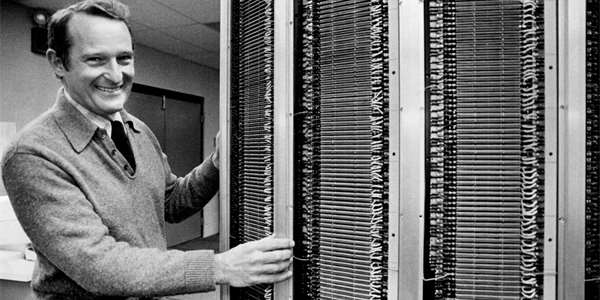
\includegraphics[width=0.5\textwidth]{Figures/seymour-cray.jpg}
	\caption{Seymour Cray \cite{Tronner20150626}}
	\label{fig:seymour-cray}
\end{figure}

Společnost Cray Research využívala ke konstrukci jejich superpočítačů až 10× rychlejší procesory v porovnání s procesory využívanými pro komerční počítače této doby. Později, počátkem 90. let 20. století se však do popředí dostávají společnosti IBM a HP, které výkonem jejich superpočítačů zastiňují všechny menší firmy pokoušející se o vývoj vlastních superpočítačů.

V minulosti byly superpočítače navrhovány pro konkrétní úlohu. Příkladem takto specializovaného výpočetního clusteru je superpočítač Deep Blue, který byl vyvinut společností IBM. Jeho úkolem bylo počítat postavení šachových figur na hracím poli. Tento superpočítač měl k dispozici 64 procesorů, na každou buňku hracího pole jeden. Deep Blue byl schopen spočítat až 200 milionů postavení šachových figur za sekundu. V květnu roku 1997 tento superpočítač porazil ruského šachového velmistra Garry Kasparova \cite{Hosch20191128}.

\begin{figure}[h]
	\centering
	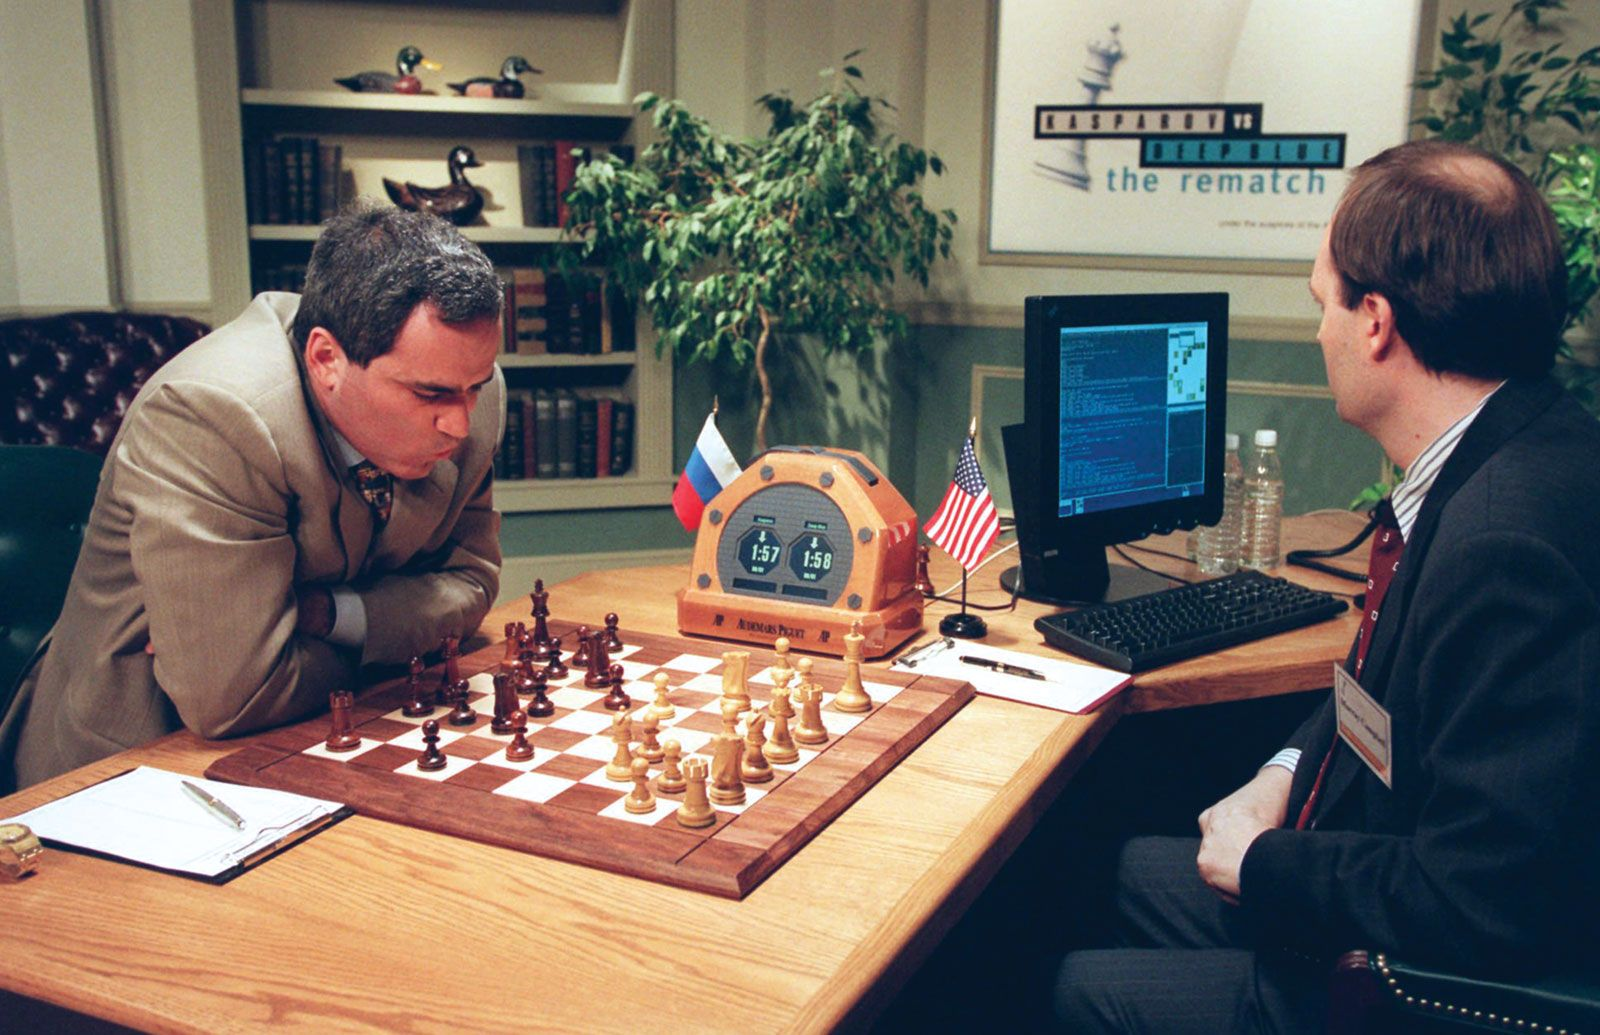
\includegraphics[width=0.5\textwidth]{Figures/Garry-Kasparov-playing-against-Deep-Blue.jpeg}
	\caption{Garry Kasparov hraje proti Deep Blue \cite{Hosch20191128}}
	\label{fig:garry-kasparov}
\end{figure}

\section{Výkon superpočítače}
Celosvětově využívanou metrikou pro měření výkonu superpočítačů je jednotka Flop/s. Jedná se \\o metriku, která je založena na počtu vykonaných operací v pohyblivé řádové čárce za sekundu. \\V době psaní této práce nejvýkonnější superpočítače světa dosahují výkonu přes 440 PFlop/s.

Dle světového žebříčku TOP500 je nejvýkonnějším superpočítačem v této době 
„Supercomputer Fugaku“ s ověřeným praktickým výkonem 442010 TFlop/s. Teoretický výkon tohoto clusteru je pak přes 537 PFlop/s, je počítán z udávaných hodnot frekvence použitých procesorů. Tento superpočítač má k dispozici přes 7,5 milionu jader a vlastní jej největší japonská vědecká instituce RIKEN \cite{B2TvJy8L3mSIxfWp}.

Nejvýkonnějším superpočítačem v České republice je nyní cluster Karolina s celkovým teoretickým výkonem 3,8 PFlop/s \cite{oviOzaWRPKlKSq7K}. Tento výpočetní cluster je umístěn v národním superpočítačovém centru IT4Innovations při Vysoké škole báňské – Technické univerzitě Ostrava. Superpočítač Karolina je v době psaní této práce umístěn na 71. pozici ve světovém žebříčku TOP500 \cite{iqgLoV1cXM0Qb6t1}.

Vývoj v odvětví IT se však žene stále kupředu a je jen otázkou času, kdy se v žebříčku objeví nový superpočítač a opětovně celým pořadím zamíchá.

\section{Plánovač úloh}
Výpočetní cluster je z praktického hlediska implementací dávkového systému. Uživatelé sami jejich programy na systému nespouští, ale dávají pokyn plánovači, který zajistí zpracování úlohy \cite{W94NKRaxvG2L2A1W}. Jedná se o program, který spravuje životní cyklus úloh na clusteru. Dle vypočtené priority řadí vytvářené úlohy do fronty, ze které jsou následně úlohy spouštěny. Stěžejními atributy pro zařazení úlohy do fronty mohou být například žádosti o množství zdrojů, doba zpracování nebo priorita úlohy.

Aby nedocházelo k plýtvání nevyužívaných zdrojů, je také jedním z hlavních faktorů zařazení úlohy do fronty využití samotných uzlů na výpočetním clusteru. Pokud tedy plánovač volí pořadí spouštění jednotlivých úloh, mezi metriky zařazuje i vlastní volné zdroje na kterých mohou být spouštěny kratší úlohy, i když pokyn k jejich zpracování přišel později než u časově náročnějších úloh.

I přes vysoký výkon superpočítačů a jejich neustálý vývoj není aktuálně možné uspokojit veškeré uživatelské požadavky ke zpracování úloh. Vytížení superpočítače a jeho zdrojů se průměrně pohybuje mezi 80-90 \%, každou dokončenou úlohu tak většinou nahrazuje úloha další. Uživatel tedy zpravidla na spuštění úlohy čeká. I tento problém pomáhá řešit plánovač na superpočítačovém clusteru. 

Následující obrázek \ref{fig:planovani-uloh} ilustruje plánování úloh s ohledem na co možná nejefektivnější využití výpočetních zdrojů. V tomto případě se jedná o dávkový systém se 6 výpočetními uzly. Cílem plánovače je zvolit pořadí spouštění úloh, tak, aby bylo minimalizováno plýtvání zdroji. Jednou \\z podmínek plánovače je omezení naplánování nanejvýš jedné úlohy na jeden uzel v jednom čase. \\V tomto příkladu se plánuje 9 úloh.

\begin{figure}[h]
	\centering
	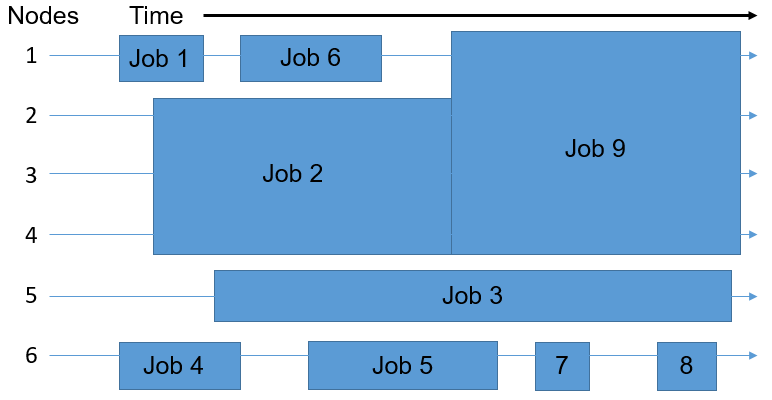
\includegraphics[width=0.7\textwidth]{Figures/Scheduler.png}
	\caption{Plánování úloh \cite{W94NKRaxvG2L2A1W}}
	\label{fig:planovani-uloh}
\end{figure}

Mezi hlavní úkoly každého plánovače se řadí zajištění spuštění každé úlohy (žádná úloha nesmí čekat ve frontě nekonečně dlouhou dobu), minimalizace nevyužití zdrojů a maximalizace průchodnosti úloh systémem.


\subsection{Plánovací algoritmy}
Jak už bylo popsáno výše, plánovač je odpovědný za řazení úloh do fronty. Další úlohou plánovače je přidělování zdrojů jednotlivým úlohám v době jejich běhu dle zásad a dostupnosti zdrojů. 

Mezi nejčastěji využívané plánovací algoritmy se řadí algoritmus zvaný FCFS (first-come first-served). Při této variantě použitého algoritmu plánovač kontroluje, zda je možné spustit první úlohu ve frontě. Tato fronta je pak v praxi označována jako fronta typu FIFO (first-in-first-out). 

K plánování HPC úloh může být také využit algoritmus ALCF (Argonne Leadership Computing Facility), princip tohoto algoritmu je obdobný jako u již zmiňovaného FCFS s rozdílem prioritizace časově náročnějších úloh a úloh, které jsou ve frontě již dlouhou dobu. 

Nejčastěji je však při plánování úloh využíváno techniky Backfilling. Technika Backfilling je optimalizovanou variantou algoritmu či principu FCFS, plánovač zkontroluje, zda je možné spustit první úlohu ve frontě. Pokud je to možné (je dostatek prostředků), úloha se spustí bez dalšího čekání. Pokud to však možné není, plánovač projde zbytek fronty a provádí kontrolu, zda je možné spustit další úlohu, aniž by se prodloužila čekací doba první úlohy ve frontě \cite{pr00bfp79qnvRTQ3}.

Na obrázku \ref{fig:fcfs-without-backfilling} je ilustrována průchodnost systémem s využitím plánovacího algoritmu FCFS bez využití techniky Backfilling. Ilustrace \ref{fig:fcfs-with-backfilling} znázorňuje taktéž algoritmus FCFS s využitím techniky Backfilling. Při porovnání těchto ilustračních obrázků je možné vidět značné omezení plýtvání zdroji a maximalizaci průchodnosti systémem při použití techniky Backfilling. Bloky s čísly znázorňují plánované úlohy z fronty. Již běžící úlohy jsou označeny jako „running job“.
\newpage
\begin{figure}
	\centering
	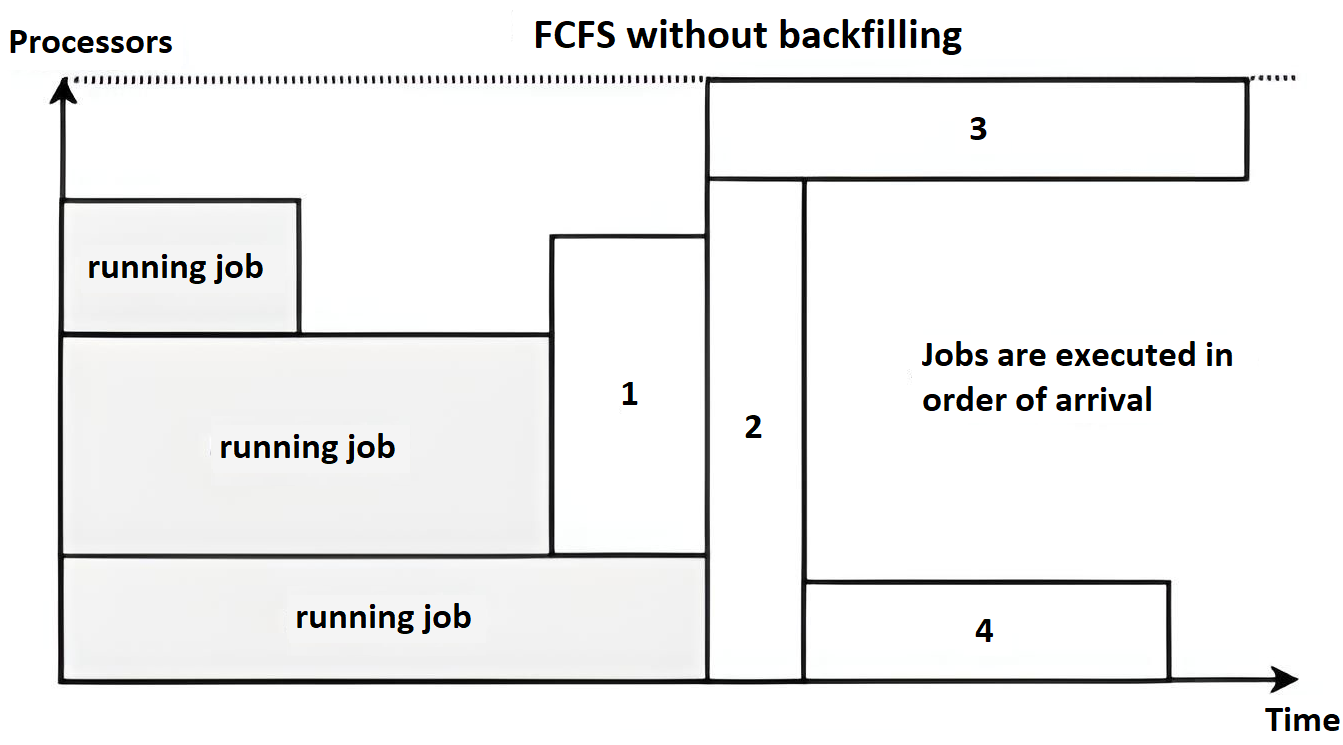
\includegraphics[width=0.8\textwidth]{Figures/fcfs-wb.png}
	\caption{Algoritmus FCFS bez použití techniky Backfilling \cite{GomezMartin2016}}
	\label{fig:fcfs-without-backfilling}
\end{figure}

\begin{figure}
	\centering
	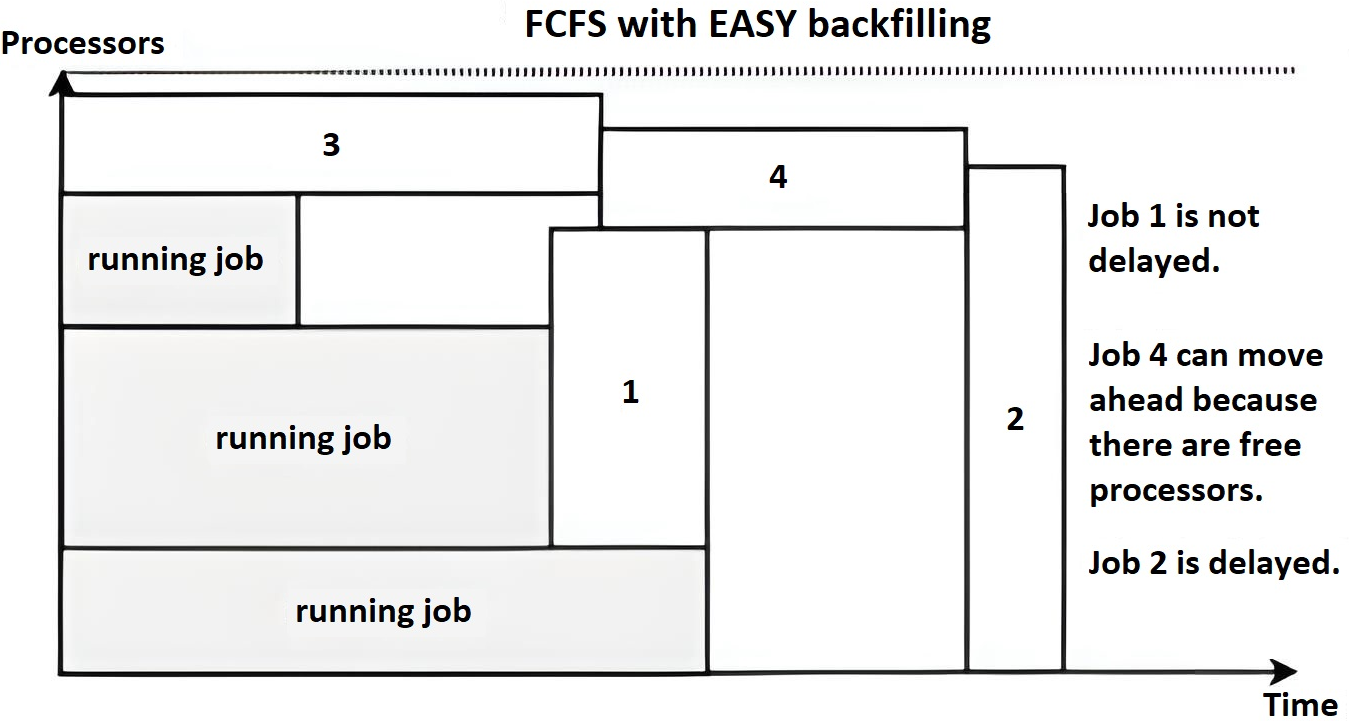
\includegraphics[width=0.8\textwidth]{Figures/fcfs-web.png}
	\caption{Algoritmus FCFS s použitím techniky Backfilling \cite{GomezMartin2016}}
	\label{fig:fcfs-with-backfilling}
\end{figure}
